% !TeX root = ../analisi_2.tex

\section{Successioni di funzioni}

\subsection{Classi di funzioni}

Per chiarire meglio le proprietà delle funzioni, è comodo parlare di classi
di funzioni.

\[
C^0 = \{f : f \text{ è continua}\}
\]

Se il dominio di $f$ è $A$, allora scriveremo

\[
f \in C^0(A).
\]

Analogamente:

\[
C^1 =
\{f : f \text{ è continua e la derivata prima è continua}\}
\]

\[
C^2 =
\{f : f \text{ è continua e le derivate prima e seconda sono continue}\}
\]

\[
C^\infty =
\{f : f \text{ è continua e tutte le sue derivate sono continue}\}.
\]


\subsection{Definizione di successione di funzioni}

\begin{definition}

Sia

\[
f_n : I \subseteq \mathbb{R} \to \mathbb{R}
\]

una successione di funzioni tutte definite in $I$.

\end{definition}


\begin{oss}

Una successione numerica è un'applicazione che ad ogni
$n \in \mathbb{N}$ associa un numero $a_n \in \mathbb{R}$:

\[
n \in \mathbb{N} \longmapsto a_n \in \mathbb{R}.
\]

Una successione di funzioni è invece un'applicazione che ad ogni
$n \in \mathbb{N}$ associa una funzione $f_n$:

\[
n \in \mathbb{N} \longmapsto f_n(x).
\]

\end{oss}


\begin{example}

Consideriamo la successione di funzioni

\[
f_n(x) = \frac{x}{n},
\qquad x \in \mathbb{R}.
\]

I primi elementi della successione sono:

\begin{align*}
f_1(x) &= x,\\
f_2(x) &= \frac{x}{2},\\
&\vdots\\
f_n(x) &= \frac{x}{n}.
\end{align*}

Fissando un valore di $x$, otteniamo una successione numerica.
Ad esempio:

\[
f_n(1) = \frac{1}{n},
\qquad
f_n(2) = \frac{2}{n}.
\]

In generale:

\[
f_n(x) = \frac{x}{n}.
\]

\begin{figure}[H]
    \centering
    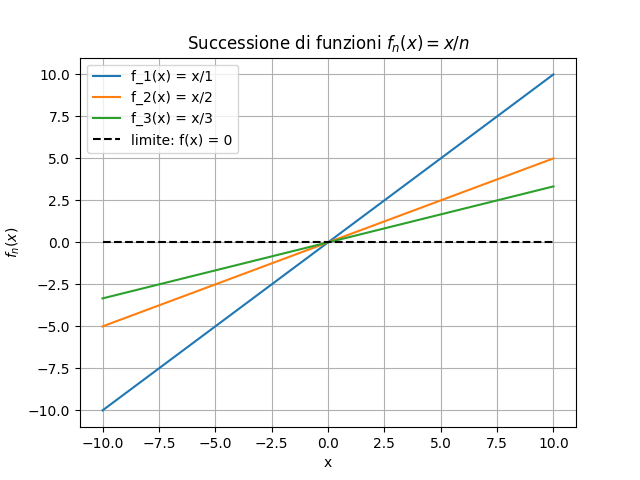
\includegraphics[width=0.5\textwidth]{./img/succ_funz_1.png}
    \caption{Grafico della successione di funzioni
    $f_n(x)=\frac{x}{n}$.}
    \label{fig:succ_funz_1}
\end{figure}

\end{example}


\begin{oss}

Viene naturale dunque domandarsi se esista una nozione di limite
per una successione di funzioni.

Fissato un $x$, la successione $f_n(x)$ è una successione numerica,
dunque posso definirne il limite

\[
\lim_{n\to\infty} f_n(x).
\]

\end{oss}


\subsection{Convergenza puntuale}

\begin{definition}

Diremo che la successione di funzioni $f_n(x)$
\textbf{converge puntualmente} alla funzione

\[
f : I \subseteq \mathbb{R} \to \mathbb{R}
\]

se

\[
\forall x \in I
\qquad
\lim_{n\to\infty} f_n(x) = f(x).
\]

Equivalentemente:
\begin{align*}
&\forall x \in I, \forall \epsilon > 0 \exists \nu_{\epsilon,x}> 0 : | f_{n} (x) - f(x) | < \epsilon \forall n > \nu_{\epsilon, x} \\
& \text{ e scriveremo } \lim_{n} f_{n} ( x) = f(x), x \in I    
\end{align*}

oppure: \(f_{n}(x) \conv{P} f(x)\) in I

\end{definition}


\begin{example}
    \[
    f_{n} (x) = \frac{x}{n} \forall x \in \R \conv{P} f(x) = 0 \forall x \in \R
    \]

    \[
    f_{n} (x) = \frac{n+x}{n+ (-1)^n + \sqrt{ n }} \conv{P} f(x) = 1
    \]
\end{example}

\begin{example}
    \[
    f_n(x) = \frac{n}{n^2x + 2n - 1}.
    \]

    Se $x=0$, il termine $n^2x$ si annulla e dunque devo distinguere
    il caso $x=0$ dal caso $x\neq 0$.

    \[
    \lim_{n\to\infty} f_n(x) =
    \begin{cases}
    0, & x \in \mathbb{R}\setminus\{0\},\\
    \dfrac{1}{2}, & x=0
    \end{cases}
    \]
\end{example}

\begin{example}
    \[
    f_{n}(x) = x^n, \; x \in [0,1]
    \]
    \[
    f_{n}(x) \conv{P} f(x) = \begin{cases}
        0, & x \in [0,1[,\\
        1, & x=1
    \end{cases}
    \]
    \begin{figure}[H]
    \centering
    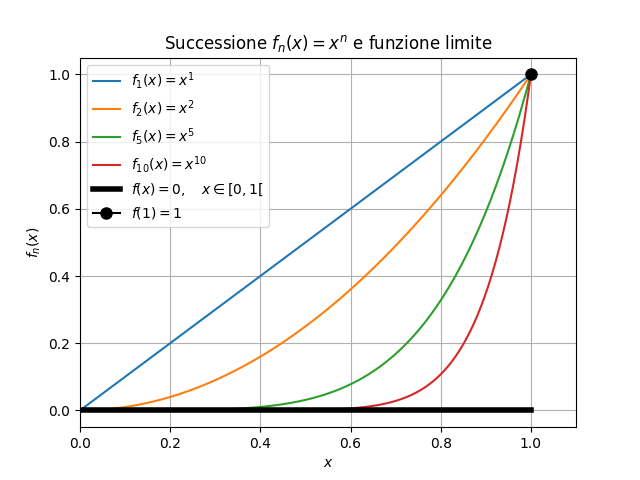
\includegraphics[width=0.5\textwidth]{./img/succ_funz_2.png}
    \caption{Grafico della successione di funzioni
    $f_n(x)=x^n$.}
    \label{fig:succ_funz_2}
    \end{figure}

\end{example}


    \begin{example}
        \[
        f_{n}(x) = x^\frac{1}{n}, \; x \in [0,1]
        \]
        \[
        f_{n}(x)\conv{P}f(x) = \begin{cases}
            1, & x \in ]0,1]\\
            0, & x =0
        \end{cases}
        \]
        \begin{figure}[H]
    \centering
    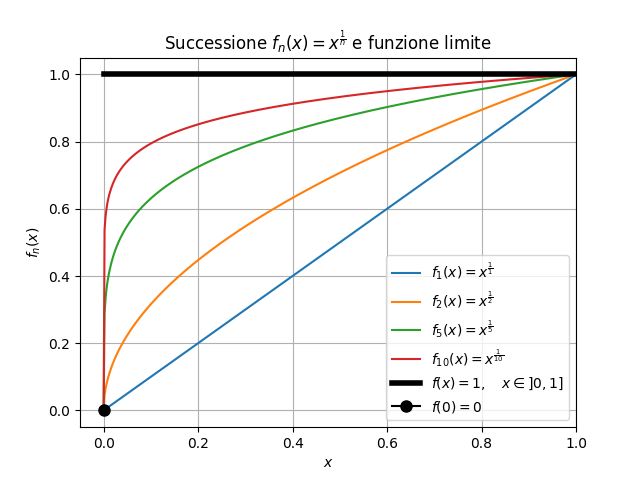
\includegraphics[width=0.5\textwidth]{./img/succ_funz_3.png}
    \caption{Grafico della successione di funzioni
    $f_n(x)=x^\frac{1}{n}$.}
    \label{fig:succ_funz_3}
    \end{figure}
        
    \end{example}

\subsection{Convergenza uniforme}

    \begin{definition}
        Sia \(f_{n}: I \sube \R \to \R, \; \forall n \in \N\)
        Diremo che \(f_{n}(x)\) \textbf{Converge Uniformemente} alla funzione \(f: I \sube \R \to \R\) e scriveremo: \(f_{n}(x)\conv{U}f(x)\) in \(I\)
        se \[\forall \epsilon > 0 \exists \nu_{\epsilon}>0 : |f_{n}(x)-f(x)| < \epsilon \, \forall n > \nu_{\epsilon}, \forall x \in I \iff\]
        \[
        \iff \forall \epsilon>0 \exists \nu_{\epsilon}>0 : \sup_{I}|f_{n}(x)-f(x)| <\epsilon \forall n > \nu_{\epsilon} \iff \lim_{n} \sup_{I}|f_{n}(x)-f(x)| = 0 \implies \lim_{n} M_{n} = 0
        \]
    \end{definition}

    \begin{example}
        \[
        f_{n} = \frac{x}{n} \conv{P} 0 \forall x\in \R \; U:?
        \]
        \[
        \sup_{\R} | \frac{x}{n} - 0| = \sup_{\R} \frac{|x|}{n} = \frac{1}{n} \sup_{\R} |x| = +\infty \implies \text{Non è Uniformemente Convergente}
        \] 
        È Unif Conv in ogni intervallo che non include una "semiretta".
    \end{example}
    \begin{example}
        \[
    f_{n}(x) = x^n, \; x \in [0,1]
    \]
    \[
    f_{n}(x) \conv{P} f(x) = \begin{cases}
        0, & x \in [0,1[,\\
        1, & x=1
    \end{cases}
    \]
    U:?
    \[
    \sup_{[0,1]} |x^n - f(x)| = 1 \not \to 0 \implies \text{Non è Unif Conv}
    \]
    È Unif Conv in \([0,b] \; 0<b<1\) 
    \end{example}

\subsection{Teorema di Continuità del Limite}
\begin{theorem}[Teo di Continuità del Limite]
    Sia \(f_{n}: I \sube\R \to \R \forall n\), una successione di funzioni continue.
    Sia \(f_{n}\conv{U} f\) in \(I\).
    Allora \(f\) è continua in I (\pencilnote{Non vale l'inversa, si pensi a \(f_{n}=\frac{x}{n}\conv{P}f=0\)}) ovvero:
    \[
    \forall x_{0} \in I \text{ si ha } \lim_{x\to x_{0}} f(x) = \lim_{x\to x_{0}}(\lim_{n\to +\infty} f_{n}(x))= f(x_{0}) =\lim_{n\to +\infty }(\lim_{x\to x_{0}} f_{n}(x)) = \lim_{n \to +\infty }f_{n}(x_{0})
    \]
    \pencilnote{Se mi voglio restringere per trovare un intervallo di uniformità, dovrò prenderne uno dove \(f(x)\) è continua.}
\end{theorem}

\begin{proof}
    Sia \(x_{0}\in I\) (\pencilnote{avendo fissato \(x_{0}\implies\)la def di continuità è \(\forall x_{0} \in I \forall \epsilon>0 \exists \delta_{\epsilon,x_{0}}\dots, \) avendolo fissato, posso scrivere \(\forall\epsilon>0\), vogliamo dimostrare che \(f\) è continua in \(x_{0}\).})
    Consideriamo le Hp:
    \begin{enumerate}
        \item \(f_{n}\) è continua in \(x_{0} \iff \forall \epsilon > 0 \exists \delta_{n}>0 : \forall x \in I, |x-x_{0}| < \delta_{n} \implies |f_{n}(x)-f_{n}(x_{0})|<\epsilon\)
        \item \(f_{n}\conv{U}f \text{ in } I \iff \forall \epsilon > 0 \exists \nu_{\epsilon}>0: |f_{n}(x)-f(x)|<\epsilon \forall n>\nu_{\epsilon}, \forall x \in I\)
    \end{enumerate}
    Th: \(\forall \epsilon>0 \exists \delta_{\epsilon}>0 : \forall x \in I, |x-x_{0}|<\delta_{\epsilon}\implies |f(x)-f(x_{0})|<\epsilon\)
    Sia \(\epsilon'>0\) e consideriamo (fissato un \(\overline{n}\) che superi la soglia)
    \begin{align*}
    &|f(x)-f(x_{0})|=|f(x)+f_{\overline{n}}(x)-f_{\overline{n}}(x)+f_{\overline{n}}(x_{0})-f_{\overline{n}}(x_{0})-f(x_{0})| \underset{\text{Dis. Tri.}}{\leq} \\ 
    &\leq \underset{(1)}{|f(x)-f_{\overline{n}}(x)|}+\underset{(2)}{|f_{\overline{n}}(x)-f_{\overline{n}}(x_{0})|}+\underset{(3)}{|f_{\overline{n}}(x_{0})-f(x_{0})|} < 3\epsilon'
    \end{align*}
\begin{oss}
\begin{enumerate}
    \item è minore di \(\epsilon'\) perchè \(f_{n}\conv{U}f\)
    \item fissato un \(\overline{n}\) se \(|x-x_{0}|<\delta_{\overline{n}}\equiv \delta_{\epsilon}\implies |f_{\overline{n}}(x)-f_{\overline{n}}(x_{0})|<\epsilon'\)
    \item analogo a (1) poichè essendo UNIFORME, vale \(\forall x \in I\)
\end{enumerate}
\end{oss}
Segue quindi \(|f(x)-f(x_{0})|<3\epsilon' \equiv \epsilon\), dunque vale la tesi.
\end{proof}


\subsection{Passaggio al limite sotto il segno di integrale}
\pencilnote{Immaginiamo di voler calcolare \(\int_{a}^{b}f(x)dx \implies \) per assicurare l'integrabilità mi serve che \(f_{n}\conv{U}f\), a questo punto \(\int_{a}^{b}\lim_{n}f_{n}(x)dx = \int_{a}^{b}f(x)dx\).

Ci chiediamo dunque se sia possibile cambiare l'ordine degli operatori, ovvero: \(\lim_{n}\int_{a}^{b}f_{n}(x)dx = \int_{a}^{b}\lim_{n}f_{n}(x)dx\)}

\begin{theorem}[Teorema Passaggio al limite sotto il segno di integrale]
    \begin{itemize}
        \item Sia \(f_{n}: [a,b]\sube\R \to \R\) continua \(\forall n\)
        \item Sia \(f_{n}\conv{U} f\) in \([a,b]\)
    \end{itemize}
    \pencilnote{(Con queste due hp mi sono assicurato la continuità di \(f\))}
    Allora: 
    \[
    \lim_{n} \int_{a}^{b} f_{n}(x) dx = \int_{a}^{b} \lim_{n} f_{n}(x) dx = \int_{a}^{b} f(x) dx
    \]
    \pencilnote{Non vale \((\impliedby)\), ovvero può valere il passaggio ma non la uniforme convergenza.}
\end{theorem}
\begin{proof}
    \pencilnote{Sia \(I_{n} = \int_{a}^{b} f_{n} (x) dx\), essa rappresenta la successione degli integrali, che essendo definiti, sono una successione numerica.}
    Per dimostrare che \(I_{n}\to I\) useremo il Teorema dei carabinieri:
    \[
    0\leq |I_{n} - I| \leq | \int_{a}^{b} f_{n}(x) - f(x) dx| \leq \int_{a}^{b} |f_{n}(x) - f(x)| dx \leq (\max_{[a,b]}|f_{n}(x) - f(x)|)(b-a)
    \]
    \pencilnote{Il massimo esiste perchè la differenza è continua in un compatto}
    A questo punto, considerando che il max esiste, esso è il sup. Sfruttiamo l'unif conv che ci dice che se \(n \to +\infty \implies sup \to 0 \) dunque:
    \[
    0 \leq \lim_{n} |I_{n} -I| \leq \lim_{n} (\max_{[a,b]}|f_{n}(x) - f(x)|)(b-a)
    \]
    Per il teo dei carabinieri, si ha che \(I_{n}\to I\)
\end{proof}


\begin{example}
    Sia \(f_{n}(x) = nx(1-x^2)^n,\; x\in[0,1]\)
    \(f_{n}(x)\conv{P}f(x)\equiv 0\) \pencilnote{è continua quindi per quello che sappiamo (escluso questo teorema), potrebbe essere unif.}
    Se integrando \(f(x)\), il valore risulta diverso da \(\lim_{n}\int_{0}^{1}f_{n}(x) dx\), allora la convergenza non è uniforme.
    \[
    \int_{0}^{1} 0 dx = 0
    \]
    \[
    \begin{aligned}
    \lim_{n\to\infty}\int_0^1 n(1-x^2)^n x\,dx
    &=\lim_{n\to\infty}\frac {n}{2}\int_0^1(1-x^2)^n2x\,dx\\
    &=\lim_{n\to\infty}\frac {n}{2}\int_0^1u^n\,du
    =\lim_{n\to\infty}\frac {n}{2}\left[\frac{u^{n+1}}{n+1}\right]_0^1\\
    &=\lim_{n\to\infty}\frac{n}{2(n+1)}
    =\boxed{\frac{1}{2}},
    \end{aligned}
    \]
    dunque la conv non è uniforme.    
\end{example}

\begin{example}
    \(f_{n}(x)=nxe^{-nx}, x \in[0,1]\)
    \pencilnote{Questo esempio dimostra che non vale l'inverso. Ovvero vale il passaggio ma non vi è unif conv.}
    \(f_{n}(x)\conv{P}f(x)\equiv 0\)
    \[
    \int_{0}^{1} f(x) dx = 0
    \]
    \[
    \lim_{n} \int_{0}^{1}nx e^{-nx} dx = \dots = \lim_{n} \left. (e^{-nx} (x+\frac{1}{n}))\right|_{1}^0 = 0
    \]
    Verifichiamo sia uniforme:
    \[
    |nx e^{-nx}|= nxe^{-nx} \implies \sup_{[0,1]} (nxe^{-nx}) = \text{\pencilnote{fai derivata e trovi max}} = \frac{1}{e} \implies \lim_{n} \sup = \frac{1}{e}
    \]
    Quindi \(f_{n}\) non conv unif.    
    
\end{example}


\subsection{Passaggio al limite sotto il segno di derivata}
\begin{theorem}[Teorema Passaggio al limite sotto il segno della derivata]
    \begin{itemize}
        \item Sia \(f_{n}:[a,b]\to \R, f_{n} \in C^1 ([a,b])\) \pencilnote{L'appartenenza a \(C^1\) non è un'hp necessaria ma facilita la dimostrazione}
        \item Sia \(x_{0}\in [a,b]: \lim_{n} f_{n}(x_{0})=l \in \R\) \pencilnote{(è conv almeno in un punto)}
        \item Sia \(g:[a,b]\to \R : f_{n}' (x) \conv{U} g(x) \text{ in } [a,b]\) \pencilnote{(\(f_{n}'\) è continua per Hp, g lo è per teo di continuità del limite)}
    \end{itemize}
    Allora:
    \begin{enumerate}
        \item \(f_{n} \conv{U} f\) in \([a,b]\)
        \item \(f\in C^1 ([a,b])\) e \(f'(x) = g(x) \iff f'(x) = \frac{d}{dx} (\lim_{n} f_{n}(x)) = \lim_{n}(\frac{d}{dx} f_{n} (x))= \lim_{n}f_{n}'(x) = g(x)\)
    \end{enumerate}
\end{theorem}
\begin{proof}
    \begin{enumerate}
        \item Costruiamo \(f\). Poiché \(f_{n}\in C^1([a,b])\), vale
        \[
        f_{n}(x) = f_{n}(x_{0}) + \int_{x_{0}}^{x} f_{n}'(t)\,dt
        \]
        \pencilnote{Posso integrare questo perché \(f_{n}'\) è continua per Hp.}
        Passando al limite per \(n\to+\infty\):
        \[
        f_{n}(x) \conv{P} l + \int_{x_{0}}^{x} \lim_{n} f_{n}'(t)\,dt = l + \int_{x_{0}}^{x} g(t)\,dt = f(x)
        \]
        \pencilnote{Il limite di \(f_{n}(x_{0})\) esiste per Hp. Poiché \(f_{n}'\conv{U} g\), posso usare il teorema di passaggio al limite sotto il segno di integrale.}
        \item Verifichiamo che vale il passaggio al limite sotto la derivata (Th 2).
        Per costruzione \(f(x) = l + \int_{x_{0}}^{x} g(t)\,dt\) con \(g\) continua, dunque per il teorema fondamentale del calcolo integrale \(f\) è derivabile e
        \[
        f'(x) = g(x),
        \]
        che è continua: quindi \(f\in C^1([a,b])\). Inoltre, per Hp, \(f_{n}'\conv{U} g = f'\).
        \item Verifichiamo che \(f_{n}\conv{U} f\) (Th 1). Per ogni \(x\in[a,b]\):
        \begin{align*}
        0 \leq |f_{n}(x)-f(x)| &= \left| f_{n}(x_{0}) - l + \int_{x_{0}}^{x} \big(f_{n}'(t) - g(t)\big)\,dt \right| \leq \\
        &\leq |f_{n}(x_{0}) - l| + \int_{x_{0}}^{x} |f_{n}'(t) - g(t)|\,dt \leq \\
        &\leq |f_{n}(x_{0}) - l| + \max_{[a,b]} |f_{n}'(x) - g(x)|\,(b-a)
        \end{align*}
        Poiché \(f_{n}'\conv{U}g\) e \(f_{n}(x_{0})\to l\), il membro di destra tende a \(0\) e non dipende da \(x\). Per il teorema dei carabinieri \(|f_{n}(x)-f(x)|\to 0\) \(\forall x\in[a,b]\); passando al sup, otteniamo che la convergenza è uniforme.
    \end{enumerate}
\end{proof}

\begin{example}
    Sia \(f_{n}(x)=\sqrt{x^{2}+\frac{1}{n}}, \; x\in\R\). Osserviamo che \(f_{n}\in C^{\infty}(\R)\) e che \(f_{n}\conv{P} f(x)=|x|\).
    La convergenza è uniforme:
    \[
    \left|\sqrt{x^{2}+\tfrac{1}{n}} - |x|\right| = \sqrt{x^{2}+\tfrac{1}{n}} - |x| = \frac{\frac{1}{n}}{\sqrt{x^{2}+\frac{1}{n}}+|x|} \leq \frac{\frac{1}{n}}{\frac{1}{\sqrt{n}}} = \frac{1}{\sqrt{n}} \to 0
    \]
    Dunque \(f_{n}\conv{U} f\), ma \(f(x)=|x|\) non è derivabile in \(0\): la convergenza uniforme di \(f_{n}\) non implica la derivabilità del limite. Ovvero, il limite di funzioni \(C^{\infty}\) può non essere nemmeno \(C^1\).
\end{example}

\begin{example}
    Sia \(f_{n}(x)=\frac{\sin(nx)}{n}\) in \(\R\), \(f_{n}\in C^{\infty}(\R)\).
    Si ha \(f_{n}\conv{P} f\equiv 0\) e la convergenza è uniforme, perché
    \[
    \left|\frac{\sin(nx)}{n}\right| = \frac{|\sin(nx)|}{n} \leq \frac{1}{n}\to 0 .
    \]
    \(f\) è derivabile. Possiamo dire che vale il passaggio? Le Hp 1 e 2 sono verificate, e l'Hp 3?
    \[
    f_{n}'(x)=\cos(nx)
    \]
    Questa è una successione che in generale non ammette limite. Inoltre, anche dove il limite esiste (ad esempio in \(x=0\)), vale \(f_{n}'(0)=1\to 1\), mentre \(f'(x)=0\).
    Ergo non vale il passaggio.
\end{example}

\begin{example}
    Sia \(f_{n}(x)=\frac{x}{1+n^{2}x^{2}}, \; x\in[0,1]\), \(f_{n}\in C^{\infty}([0,1])\).
    Si ha \(f_{n}\conv{P} f\equiv 0\). Inoltre
    \[
    f_{n}'(x)=\frac{1-n^{2}x^{2}}{(1+n^{2}x^{2})^{2}}
    \]
    e \(f_{n}'(x)\geq 0 \iff 1-n^{2}x^{2}\geq 0 \iff x\leq \frac{1}{n}\).
    Quindi il massimo di \(f_{n}\) è in \(x=\frac{1}{n}\) e
    \[
    \sup_{[0,1]} f_{n}(x) = f_{n}\left(\tfrac{1}{n}\right) = \frac{1}{2n}\to 0 \implies f_{n}\conv{U} f .
    \]
    Vale il passaggio? \(f'(x)=0\), ma
    \[
    f_{n}'(x)\conv{P}\begin{cases} 1 & x=0 \\ 0 & x\neq 0 \end{cases}
    \]
    che è discontinua: dunque \(f_{n}'\) non può convergere uniformemente (altrimenti il limite sarebbe continuo per il teorema di continuità del limite) e infatti non vale il passaggio, perché \(\lim_{n}f_{n}'(0)=1\neq 0=f'(0)\).
\end{example}


\subsection{Convergenza uniforme e discontinuità}
Finora abbiamo parlato di conservazione della continuità. La convergenza uniforme conserva anche la discontinuità?

\begin{oss}
    La convergenza uniforme \textbf{non} conserva la discontinuità: una successione di funzioni discontinue può convergere uniformemente a una funzione continua.
\end{oss}

\begin{example}
    Sia
    \[
    f_{n}(x)=\begin{cases} \frac{1}{n} & x\in\mathbb{Q} \\ 0 & x\in\R\setminus\mathbb{Q} \end{cases}
    \]
    Ogni \(f_{n}\) è discontinua in ogni punto per la densità di \(\mathbb{Q}\) in \(\R\).
    Si ha \(f_{n}\conv{P}0\) in \(\R\) e \(f_{n}\conv{U}0\) in \(\R\) \pencilnote{(per dimostrare l'uniforme basta osservare che il sup è \(\frac{1}{n}\to 0\))}.
\end{example}


\subsection{Criterio di Cauchy}
\subsubsection{Criterio di Cauchy per la convergenza puntuale}
\begin{theorem}[Criterio di Cauchy per la convergenza puntuale]
    Sia \(f_{n}:I\sube\R\to\R\) \(\forall n\in\mathbb{N}\) e sia \(f:I\sube\R\to\R\).
    \[
    f_{n}\conv{P}f \text{ in } I \iff \forall x\in I,\; \forall\epsilon>0\; \exists \nu_{\epsilon,x}>0 : |f_{n}(x)-f_{m}(x)|<\epsilon \quad \forall n,m>\nu_{\epsilon,x}
    \]
\end{theorem}
\begin{proof}
    Segue dal criterio di Cauchy per le successioni numeriche, poiché fissata una \(x\in I\), \(f_{n}(x)\) è una successione numerica.
\end{proof}

\subsubsection{Criterio di Cauchy per la convergenza uniforme}
\begin{theorem}[Criterio di Cauchy per la convergenza uniforme]
    Sia \(f_{n}:I\sube\R\to\R\) \(\forall n\in\mathbb{N}\) e sia \(f:I\sube\R\to\R\).
    \[
    f_{n}\conv{U}f \text{ in } I \iff \forall\epsilon>0\; \exists \nu_{\epsilon}>0 : |f_{n}(x)-f_{m}(x)|<\epsilon \quad \forall n,m>\nu_{\epsilon},\; \forall x\in I
    \]
    \pencilnote{Ogni volta che fisso una \(x\) in \(I\), ottengo una successione di Cauchy con lo stesso \(\nu\).}
\end{theorem}
\begin{proof}
    \((\implies)\) Se \(f_{n}\conv{U}f\) in \(I\), allora \(\forall\epsilon>0\; \exists\nu_{\epsilon}: |f_{n}(x)-f(x)|<\epsilon\) \(\forall n>\nu_{\epsilon}\), \(\forall x\in I\).
    Allora
    \[
    |f_{n}(x)-f_{m}(x)| = |f_{n}(x)-f(x)-f_{m}(x)+f(x)| \underset{\text{Dis. Tri.}}{\leq} |f_{n}(x)-f(x)|+|f_{m}(x)-f(x)| < 2\epsilon
    \]
    da cui la tesi. Se \(n,m>\nu_{\epsilon}\) e \(\forall x\in I\) otteniamo che i moduli sono \(<\epsilon\) per Hp.

    \((\impliedby)\) Supponiamo che \(\forall\epsilon>0\; \exists\nu_{\epsilon}>0: |f_{n}(x)-f_{m}(x)|<\epsilon\) \(\forall n,m>\nu_{\epsilon},\; \forall x\in I\) \hfill \((*)\) \pencilnote{(vale la condizione di Cauchy)}

    Fissata una \(x\in I\), la successione \(f_{n}(x)\) è una successione numerica di Cauchy che converge a un certo numero reale \(f(x)\). Possiamo quindi scrivere
    \[
    |f_{n}(x)-f(x)| = \lim_{m\to+\infty} |f_{n}(x)-f_{m}(x)|
    \]
    Dunque, passando al limite per \(m\to+\infty\) nella condizione di Cauchy \((*)\), otteniamo
    \[
    \forall\epsilon>0\; \exists\nu_{\epsilon}>0: |f_{n}(x)-f(x)|\leq\epsilon \quad \forall n>\nu_{\epsilon},\; \forall x\in I,
    \]
    cioè \(f_{n}\conv{U}f\) in \(I\).
\end{proof}
